\documentclass{article}%
\usepackage[T1]{fontenc}%
\usepackage[utf8]{inputenc}%
\usepackage{lmodern}%
\usepackage{textcomp}%
\usepackage{lastpage}%
\usepackage[head=40pt,margin=0.5in,bottom=0.6in]{geometry}%
\usepackage{graphicx}%
%
\title{\textbf{Vecinos de Chacao se organizan ante las malas condiciones del agua}}%
\author{Giselle Goncalves | @GiselleAGP}%
\date{17/10/2018}%
%
\begin{document}%
\normalsize%
\maketitle%
\textbf{URL: }%
http://www.el{-}nacional.com/noticias/servicios/vecinos{-}chacao{-}organizan{-}ante{-}las{-}malas{-}condiciones{-}del{-}agua\_256205\newline%
%
\textbf{Periodico: }%
EN, %
ID: %
256205, %
Seccion: %
Servicios\newline%
%
\textbf{Palabras Claves: }%
Hidrocapital, Agua, Caracas, Denuncia\newline%
%
\textbf{Derecho: }%
3.2, %
Otros Derechos: %
2.8, %
Sub Derechos: %
3.2.1, 2.8.1\newline%
%
\textbf{EP: }%
NO\newline%
\newline%
%
\textbf{\textit{Gabriel Santana, dirigente vecinal, dio consejos para mejorar el estado del agua antes de consumirla}}%
\newline%
\newline%
%
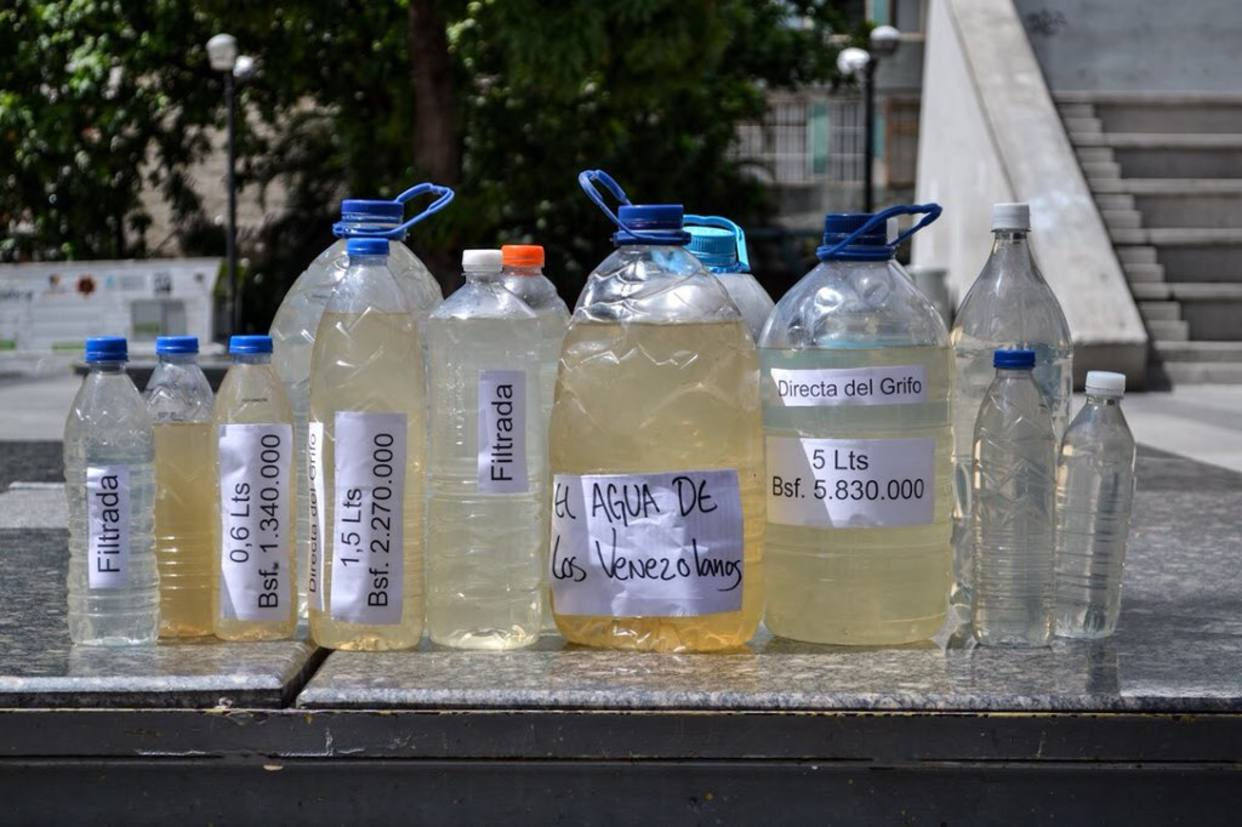
\includegraphics[width=300px]{54.jpg}%
\newline%
%
La mala calidad del servicio de agua se ha convertido en una cotidianidad para los venezolanos. Los ciudadanos han adaptado su rutina ante la incertidumbre de cuándo volverán a contar con este recurso de una manera regular.%
\newline%
%
En el municipio Chacao inició este miércoles una campaña que pretende educar a los afectados por esta situación, que son la mayoría de los habitantes del país. Gabriel Santana, dirigente vecinal, es el promotor de este movimiento que ayuda a las comunidades para que encuentren soluciones temporales.%
\newline%
%
Actualmente, la insuficiente constancia de la circulación del agua en la ciudad y sus condiciones preocupan a los vecinos del municipio. Desde diversos estados, los venezolanos también han mostrado en las redes sociales la precaria salubridad del agua que utilizan para el consumo.%
\newline%
%
Santana explicó, en una entrevista exclusiva para~El Nacional Web, ~que esta iniciativa tiene como objetivo enseñarles a las personas qué hacer ante este escenario reconociendo que Hidrocapital, compañía responsable del servicio del agua, está incapacitada para brindar las soluciones adecuadas.%
\newline%
%
El dirigente vecinal, junto a los vecinos de Chacao, ha realizado denuncias con respecto a la calidad del agua que llega a sus hogares, demostrando que su color y sus componentes pueden contener bacterias y virus que produzcan salmonera o distintos tipos de hepatitis. Recalcó que estos datos se han sometido a estudios~en los laboratorios de la Universidad Central de Venezuela.%
\newline%
%
"No es tan fácil porque en el laboratorio de la UCV no tienen reactivos y en los laboratorios privados se hace muy caro. Pero ya pronto tendremos una solución", dijo Santana.%
\newline%
%
Basado en estos estudios, en sugerencias de las organizaciones internacionales relacionadas con el derecho al acceso al agua, además de una recolección de opiniones de los vecinos se determinaron las técnicas para que el consumo del agua en los hogares sea más sano.%
\newline%
%
El dirigente vecinal enfatizó que este hecho debe ser denunciado ante Hidrocapital debido a que es una violación de derechos humanos que dejen que el agua llegue a las casas de los venezolanos en condiciones que impliquen un riesgo a la vida.%
\newline%
%
“Es una violación a los derechos humanos, y hay que hacer hincapié en que el responsable es Hidrocapital”, resaltó Santana.%
\newline%
%
\end{document}